\section{Organisations existantes}
Il sera présenté ici un ensemble d'initiatives similaires à ce travail. Elles sont toutes non gouvernementales et propose d'enseigner la programmation de différentes manières.
\subsection{Code.org}
\begin{figure}[!ht]
  \begin{center}
    
\includegraphics[scale=0.5]{content/5-related_work/images/code}
    \caption{Logo de code.org}
    \label{fig:code.org}
  \end{center}
\end{figure}
Code.org \cite{code-org-about} est une organisation sans but lucratif des USA qui à pour objectifs :
\begin{itemize}
  \item apporter l'informatique dans toutes les classes de secondaire aux États-Unis ;
  \item démontrer le succès de l'utilisation de cours en ligne dans l'enseignement public ;
  \item ajouter l'informatique dans les bases des programmes de sciences et de mathématique des 50 états ;
  \item employer la connaissance technique collective pour améliorer l'apprentissage de l'informatique dans le monde ;
  \item augmenter la représentation féminine et de personnes de couleurs dans l'informatique.
\end{itemize}

Pour ce faire, Code.org fourni une plate-forme \cite{code-org-20hr} web qui permet aux professeurs de suivre leurs élèves grâce à un système de classes. Ce programme d'apprentissage se base sur Blockly (voir \ref{blockly}).

Toutes les ressources sont gratuites et librement utilisables \cite{code-org-faq}. Elles sont conçues pour que les professeurs comme les étudiants puissent commencer le cours sans connaître l'informatique (une assistance gratuite est proposée au professeur si nécessaire).

Le site propose aux professeurs de se faire récompenser s'ils arrivent à finir les 27 missions proposées avec minimum 15 étudiants. Dans ce cas, ils gagnent $750\$$. S'ils ont au moins 7 filles dans le groupe, ils peuvent prétendre à $250\$$ supplémentaires.

\subsubsection{Déroulement des leçons}
Code.org propose des sessions d'une heure de travail/jeu/apprentissage. Chaque unité est découpée en missions courtes (ex:5-20) apportant un concept de programmation. Avant chaque concept, une petite vidéo l'introduit et donne des exemples d'utilisations.

Il propose de faire travailler les étudiants en binôme \cite{wiki-pair-prog}, ce qui entraîne moins de questions au professeur et permet de mieux s'approprier la matière. Le travail par binôme casse également l'image du "geek" et montre que la programmation est une science sociale et collaborative. De plus, moins d'ordinateurs sont nécessaires.

Le site explique également que pour faire participer tous les élèves, il faut avoir confiance en leur compétence. Leur philosophie est d'inciter les premiers groupes à aider les derniers.

Quand un étudiant a une question, Code.org recommande de la soumettre à 3 de ses camarades avant de la poser au professeur. Cela permet aussi d'évité les questions de distraction ou de manque de compréhension.

Pour chaque petite mission, un test automatisé informe si la mission est réussie ou non. Si celle-ci est réussie, le programme passe à la mission suivante. Dans les premières missions, il y a également un compteur de blocs qui informe du nombre de blocs nécessaires pour réaliser la mission de manière optimale.

\subsection{CoderDojo}
\begin{figure}[!ht]
  \begin{center}
    
\includegraphics[scale=0.5]{content/5-related_work/images/dojo}
    \caption{Logo de CoderDojo}
    \label{fig:coder dojo}
  \end{center}
\end{figure}
CoderDojo \cite{dojo-about} est un réseau open source de Clubs de programmation dans le sens le plus large du terme. Tous les dojos sont donc autonomes. Des enfants de 5 à 17 ans y apprennent la programmation (site web, application, jeux...). La seul règle est "Above All : Be Cool" qui est mise en pratique en créant simplement des espaces d'échanges de savoir amicaux et sociables.

CoderDojo a été créé par James Whelton, un irlandais de 18 ans, et Bill Liao, un entrepreneur australien à Cork. James, après avoir hacké l'iPod nano, a eu des demandes de jeunes enfants pour avoir des cours de programmation. Beaucoup de gens de Dublin ont été à ses cours et donc un nouveau Dojo y a été créé. Ensuite, cela s'est étendu à tout le globe.

\subsection{Code Club}
\begin{figure}[!ht]
  \begin{center}
    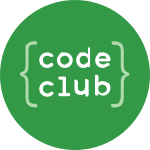
\includegraphics[scale=0.3]{content/5-related_work/images/club}
    \caption{Logo de Code Club}
    \label{fig:code club}
  \end{center}
\end{figure}
Code Club\cite{codeclub-about} est un réseau national de Clubs mené par des bénévoles en dehors des heures de cours. Leurs activités s'adressent à des enfants de 9 à 11 ans.

Ils créent le matériel pour permettre à des bénévoles de donner des cours parascolaires d'environ une heure par semaine. Ils proposent d'utiliser dans cet ordre scratch, HTML/css et puis Python. Ils ont pour objectif que les 21000 écoles fondamentales anglaises aient leur club.

Leur philosophie est de d'abord l'amusement, la créativité et l'exploration avant l'apprentissage des concepts de programmation.

\subsection{KidsCode}
\label{init-kidscode}
\begin{figure}[!ht]
  \begin{center}
    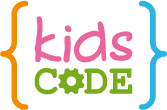
\includegraphics[scale=0.5]{content/5-related_work/images/kidscode}
    \caption{Logo de KidsCode}
    \label{fig:kidscode}
  \end{center}
\end{figure}
KidsCode \cite{kidscode} est une petite initiative wallonne qui organise actuellement un stage pour les enfants de 10 à 14 ans. Les ateliers sont dispensés par deux informaticiens qui proposent de partager leur passion. Ils encadrent les jeunes de manière ludique dans le but de les rendre autonomes.

KidsCode propose d'apprendre la programmation grâce au langage Python. Ce langage a été choisi pour sa facilité tout comme pour son utilisation en condition réelle. 

KidsCode a été conçu et pensé en association avec l'incubateur de startup Nestup. Cette initiative est le fruit du constat par les entreprises, d'un manque d'intérêt pour la programmation chez les plus jeunes. Ce qui entraîne un manque de vocation dans les startups.
